%=========================================================================
% sec-opts-loop
%=========================================================================

\section{Changing Loop Ordering}
\label{sec-opts-loop}

% Reason for optimization
\subsection{Reason for Optimization}

The memory access pattern for DGEMM is largely determined by the order in
which the matrices are traversed. Depending on the loop order and the
arrangement of the matrices in memory (i.e., row-major vs. column-major),
memory could be accessed with a unit-stride that maximizes temporal and
spatial locality, or a stride equal to the matrix dimensions that is more
likely to cause cache misses.
\smallskip

The goal of this optimization is to find the loop ordering that uses the
data in a cache line as much as possible before bringing in another cache
line. We explore a variety of loop orderings based on an intuitive
analysis of how to achieve unit-stride memory accesses to identify the
optimal loop ordering.
\smallskip

% Details of optimization
\subsection{Details of Optimization}

%=========================================================================
% fig-opts-loop-access.tex
%=========================================================================

\begin{figure}[b]

  \centering
  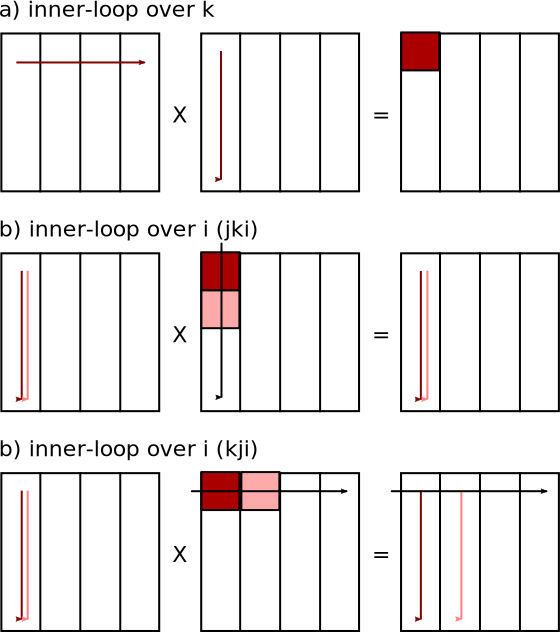
\includegraphics[width=0.5\tw]{fig-opts-loop-access.svg.pdf}

  \caption{\textbf{Memory Access Patterns of Loop Orderings --} The
    memory access patterns for the innermost loop for {\tt{ijk}},
    {\tt{jki}}, and {\tt{kji}} orderings are shown in dark red. For the
    latter two orderings, the light red arrows show the change in the
    accesses with each iteration of the middle loop. Note that {\tt{jki}}
    can reuse the data in the cache for both {\tt{B}} and {\tt{C}},
    whereas {\tt{kji}} can only reuse the data in the cache for
    {\tt{A}}. }

  \label{fig-opts-loop-access}

\end{figure}


The naive loop ordering of {\tt{ijk}} iterates across the output matrix
{\tt{C}}, traversing the columns before traversing the rows. Computing
each element in the output matrix requires traversing the columns of
{\tt{A}} and traversing the rows of {\tt{B}}. This type of access pattern
is generalized in Figure~\ref{fig-opts-loop-access}.
\smallskip

Because the matrices are arranged in a column-major pattern in memory,
it is always preferable to traverse the rows (i.e., vertically) to yield
unit-stride memory accesses. Any time we traverse the columns (i.e.,
horizontally), we only use a single element in a cache line before
accessing another cache line, which makes it more likely to have cache
misses.
\smallskip

Given this, we can see that the naive loop ordering actually generates a
very hostile memory access pattern since the innermost loop always
traverses the columns of {\tt{A}} and the middle loop traverses the
columns of {\tt{C}}.
\smallskip

Fortunately, we can leverage this insight to make an educated guess about
which loop ordering would be preferable. Since the memory access pattern
of the innermost loop is the most critical in exploiting temporal
locality, it makes sense to iterate across {\tt{i}} for the innermost
loop, as this will allow us to traverse the rows of both {\tt{A}} and
{\tt{C}}, while using a single element from {\tt{B}} to calculate the
partial products for an entire column of {\tt{C}}. Note that if the block
size is large, traversing the rows will still require accessing multiple
cache lines, but accessing consecutive cache lines will help avoid
conflict misses more than if we traversed the columns. This means that
either the {\tt{jki}} or the {\tt{kji}} ordering will yield the most
desirable memory access patterns. The former allows us to reuse the same
data for {\tt{B}} and {\tt{C}} while only shifting one column over in
{\tt{A}}, whereas the latter only allows us to reuse the same data in
{\tt{A}}. See Figure~\ref{fig-opts-loop-access} for visual comparisons.
\smallskip

% Results and analysis
\subsection{Results}

%=========================================================================
% fig-opts-loop-results.tex
%=========================================================================

\begin{figure}

  \centering
  \includegraphics[width=0.7\tw]{fig-opts-loop-results.pdf}

  \caption{\textbf{Performance Comparison of Loop Order Optimizations --}
    We intentionally omit the results for BLAS nad MKL implementations in
    order to focus on the behavior at the performance range of the
    optimization.}

  \label{fig-opts-loop-results}

\end{figure}


The results of all possible loop orderings are shown in
Figure~\ref{fig-opts-loop-results}. We only show the effects of changing
the loop ordering of the computation kernel operating on a given
block. Although we did experiment with changing the loop ordering of the
outer loop that traverses the blocks, the effects on performance were
negligible. This was slightly contrary to expectations as the order in
which the blocks are traversed should impact the reuse of data in
lower-level caches (e.g., L2, L3), whereas the loop ordering of the
computation kernel is more focused on L1 cache utilization.
\smallskip

As expected, the {\tt{jki}} ordering shows the greatest improvement in
performance, followed by the {\tt{kji}} ordering. The other orderings
either exacerbate the sub-optimal memory access patterns or have
negligible improvements over the naive ordering.
\smallskip

One caveat with not iterating over {\tt{k}} in the innermost loop is that
we cannot accumulate the partial products for a given element in the
output matrix in the local register storage. For example, in the
{\tt{jki}} ordering, we must store the partial product for all elements
in a given column in the output matrix to memory, then load each one back
again for the accumulation when {\tt{k}} increments. However, since using
the optimal loop ordering encourages reuse of data in the L1 cache, the
overhead of storing/loading of partial products is not as significant as
if we were using the naive loop ordering.
\medskip

\clearpage
